	O \textit{software} de computadores é a tecnologia mais importante no palco mundial, pelo fato de ter assumido um duplo papel; é o produto e, ao mesmo tempo o veículo para entrega do produto. Como produto, é um transformador de informações - produzindo, gerindo, modificando e exibindo informações que podem ser tão simples como um \textit{bit} ou tão complexas quando uma vídeo aula. Como veículo, o \textit{software} age como base para controlar o computador (sistemas operacionais),  para a comunicação da informação (redes de computadores) e para criação e controle de outros programas (ferramentas e ambientes de desenvolvimento)~\cite{engsoftware}.

	Com toda esse importância,  a área de desenvolvimento de \textit{softwares} cresceu de forma avassaladora, exigindo assim uma padronização, haja vista que todo sistema (\textit{software}) necessita de reparos e melhorias à medida que o tempo passa. Por estes motivos surge a engenharia de \textit{software}, que é um conjunto de métodos e ferramentas que auxiliam no projeto, desenvolvimento, testes e manutenção de um \textit{software}.

\section{Modelo de Processo de Software}
	O modelo de desenvolvimento de software utilizado neste projeto foi o incremental. Ele consiste em um processo iterativo, que objetiva entregar o produto operacional a cada incremento~\cite{engsoftware}.

	Os primeiros incrementos são versões simplificadas do produto final, que oferecem capacidades mínimas de utilização por parte do usuário. A figura~\ref{fg:engsoftware} ilustra como este modelo se comporta durante o tempo estimado para o projeto.
\begin{figure}[ht!]
	\centering
	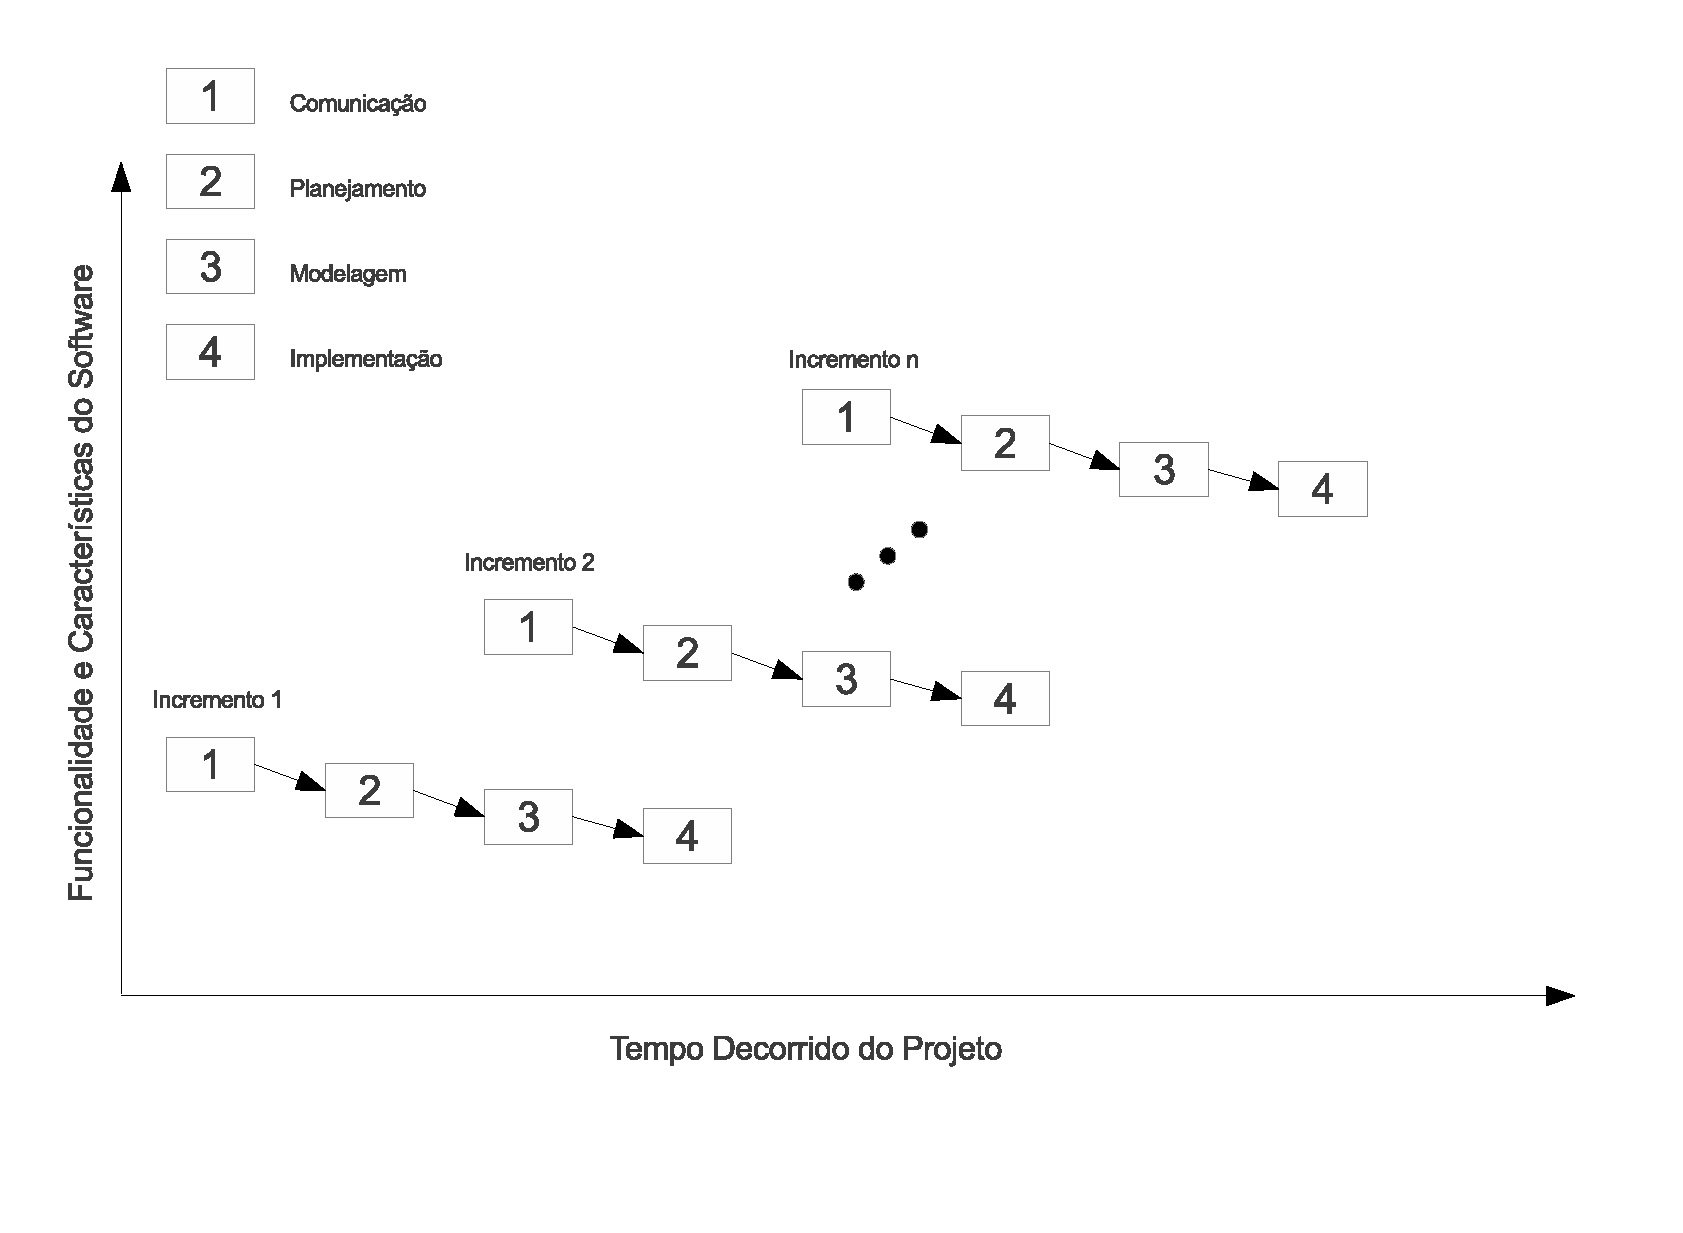
\includegraphics[scale=0.5]{engsoftware}
	\caption{Diagrama do modelo de desenvolvimento incremental.}
	\label{fg:engsoftware}
\end{figure} 

	Estão descritas abaixo, as etapas deste modelo:
\begin{enumerate}
	\item \textbf{Comunicação:} é responsável pelo levantamento do(s) propósito(s) do projeto.
	\item \textbf{Planejamento:} tem o papel de definir os requisitos do trabalho.
	\item \textbf{Modelagem:} define as ferramentas, linguagens, etapas a serem desenvolvidas.
	\item \textbf{Construção:} é o processo de codificação e testes.
	\item \textbf{Implementação:} responsável pela entrega do protótipo (inicial ou final).
\end{enumerate}

\section{Tecnologias de Programação Usadas}
	As tecnologias de programação usadas neste projeto foram: o motor de jogos \textit{Irrlicht}, a plataforma \textit{Qt-Creator} e a linguagem C++. 

	O \textit{Irrlicht} é uma máquina de jogo de alta performance escrita em linguagem C++\cite{irrlichtbook}.  Tem no fato de ser \textit{open source}~(código aberto), uma das suas principais vantagens em relação a outras \textit{engines}~(proprietárias). Abaixo estão listadas, outras características deste motor gráfico~\cite{irrlicht}. 
\begin{enumerate}
\item Renderização em tempo real de alta performance usando \textbf{Direct3D} e \textbf{OpenGL}.
\item Independe de plataforma.
\item Renderiza diretamente de arquivos, tais como : .zip, .pak, .pk3, etc.
\item Rápida e fácil detecção de colisão.
\item Possibilita o uso de vários linguagens de programação, como : C/C++, Java, Delphi, entre outras.
\item É limpa, fácil de entender, e bem documentada.
\end{enumerate}

	 O \textit{Qt-Creator} é um poderoso ambiente multi plataforma que permite a criação de diversas aplicações \textit{web} e também \textit{desktop}. Sua importância, neste trabalho, está relacionada com oferecer suporte para a criação de uma interface \textit{desktop}, a qual pudesse ser usada em diferentes sistemas operacionais~(Linux, Windows ou Macintoch) e com arquiteturas dissemelhantes~(32 ou 64 bits), para modelar tanto objetos 3D básicos como ambientes \textit{indoor}. 

	O C++ é uma linguagem orientada a objeto utilizada por milhares de programadores em inúmeros domínios de aplicação. Ela é sustentada por um conjunto vasto de bibliotecas, livros, revistas técnicas e conferências. É tão robusta que está presente no desenvolvimento (total ou de partes) de muitos sistemas operacionais. 

	Tanto as plataformas (\textit{Irrlicht} e \textit{Qt}) quanto a linguagem de programação C/C++, foram escolhidas por serem muito usadas pelo comunidade desenvolvedora por mostrarem robustez,  boa documentação e  terem uma conexão~(tanto o \textit{Irrlicht} quanto o \textit{Qt} usam a linguagem C++).

\section{Classes}
	O uso do conceito de classes, na implementação deste trabalho, se dá ao fato de que a linguagem C++ baseia-se no paradigma da orientação a objeto. A orientação a objeto é um conjunto de conceitos no qual o desenvolvimento (analise, projeto e programação) de sistemas de software está baseada na composição e iteração entre diversas unidades de software chamadas de objetos. Alguns de seus conceitos essenciais são:

\begin{itemize}
	\item \textbf{Classe}: representa um conjunto de objetos com características afins. Uma classe define o comportamento dos objetos através de seus métodos, e quais estados ele é capaz de manter através de seus atributos.
	\item \textbf{Objeto}: um objeto é capaz de armazenar estados através de seus atributos e reagir a mensagens enviadas a ele, assim como se relacionar e enviar mensagens a outros objetos.
	\item \textbf{Atributos}: são elementos que definem a estrutura de uma classe.
	\item \textbf{Métodos}: especificam a forma como os dados de um objeto são manipulados.
	\item \textbf{Herança}: é um princípio que permite que classes compartilhem atributos e métodos.
\end{itemize}

	As classes criadas para este projeto foram: \textit{IrrViewer, Cena, IrrNode, ReceiverEvent} e \textit{MainWindow}. O diagrama \textit{uml} mostrado na Figura ~\ref{fg:classes}, está representando o relacionamento entres estas classes.

\begin{figure}[ht!]
	\centering
	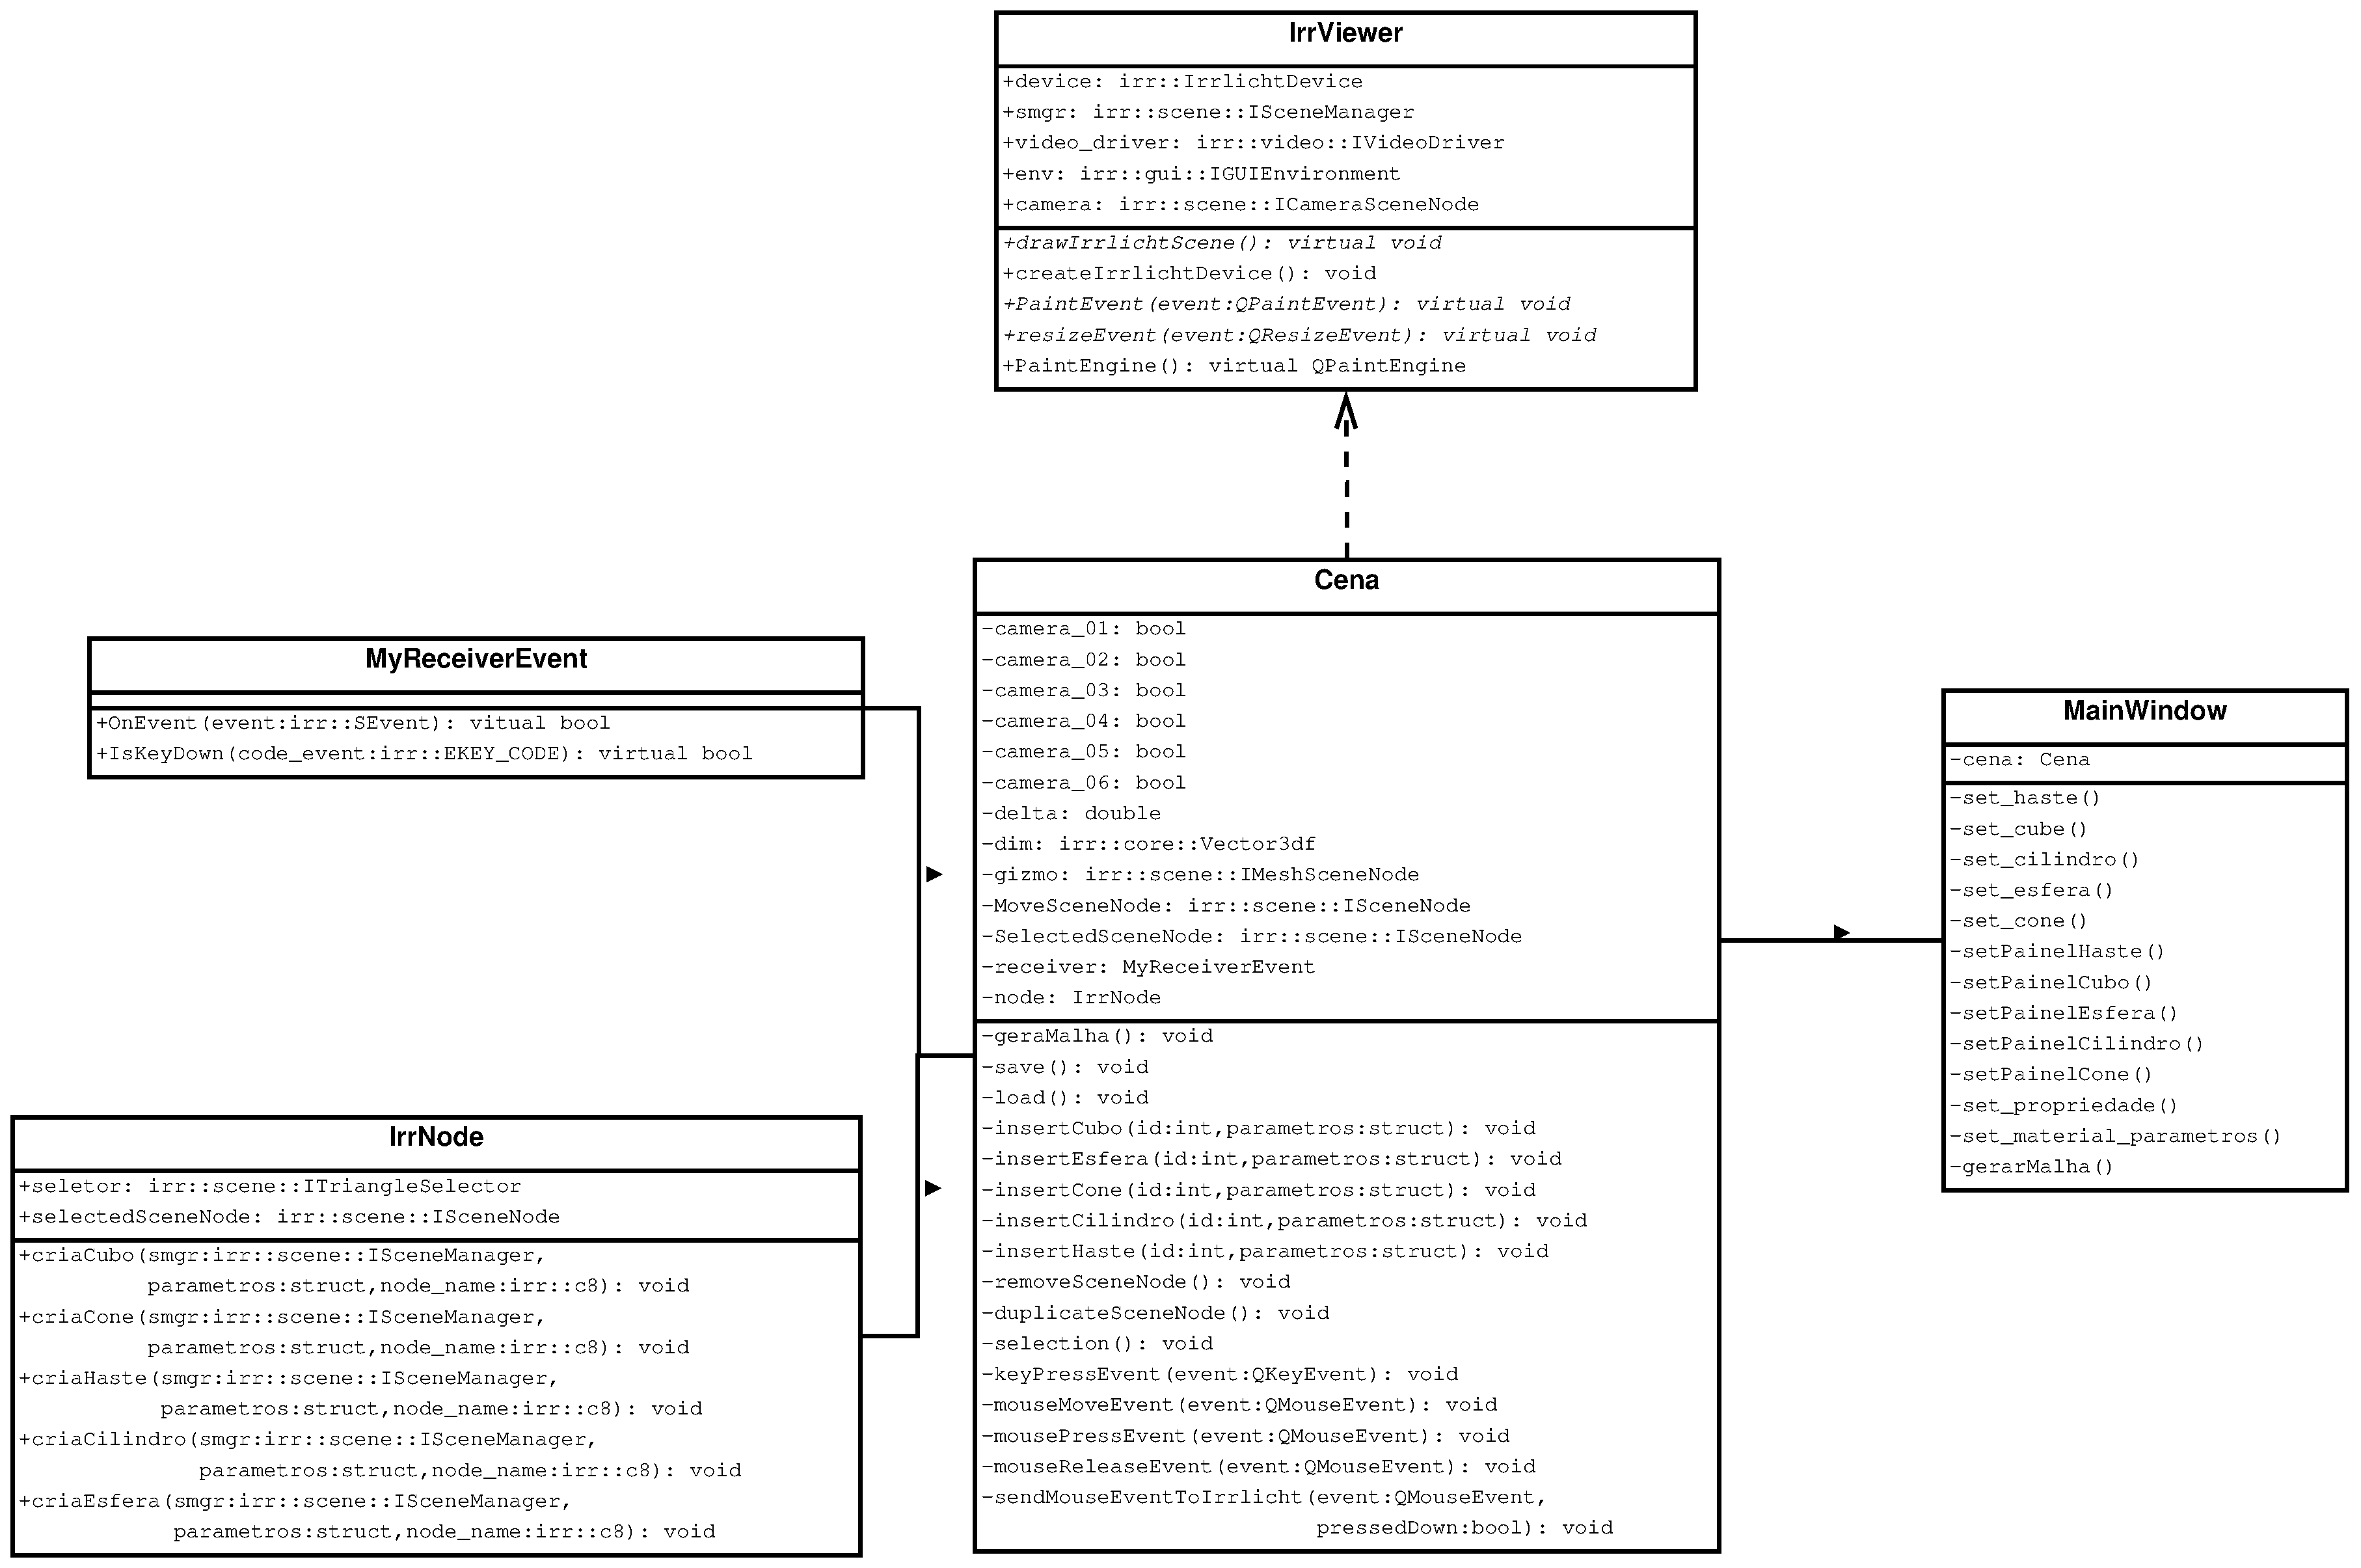
\includegraphics[scale=0.25]{classes}
	\caption{Diagrama \textit{uml} do relacionamento das classes desenvolvidas neste projeto.}
	\label{fg:classes}
\end{figure} 

	O primeiro passo no desenvolvimento deste trabalho foi a união do motor de jogos \textit{Irrlicht} com a plataforma \textit{Qt-Creator}, necessitava-se que a cena \textit{Irrlicht} fosse reconhecida como uma janela padrão do \textit{Qt} (para poder introduzi-la na interface ). Para tanto, foi necessário o estudo das classes básicas destes dois universos, assim como suas principais características. 

	Esta união foi concretizada por meio da criação da classe \textit{IrrViewer}, que contêm tantos os métodos que caracterizam uma classe \textit{Widget} quanto os necessários para criação de um cenário \textit{Irrlicht}. A Figura~\ref{fg:classeirrviewer} ilustra os principais atributos e métodos desta classe.
\begin{figure}[!ht]
	\centering
	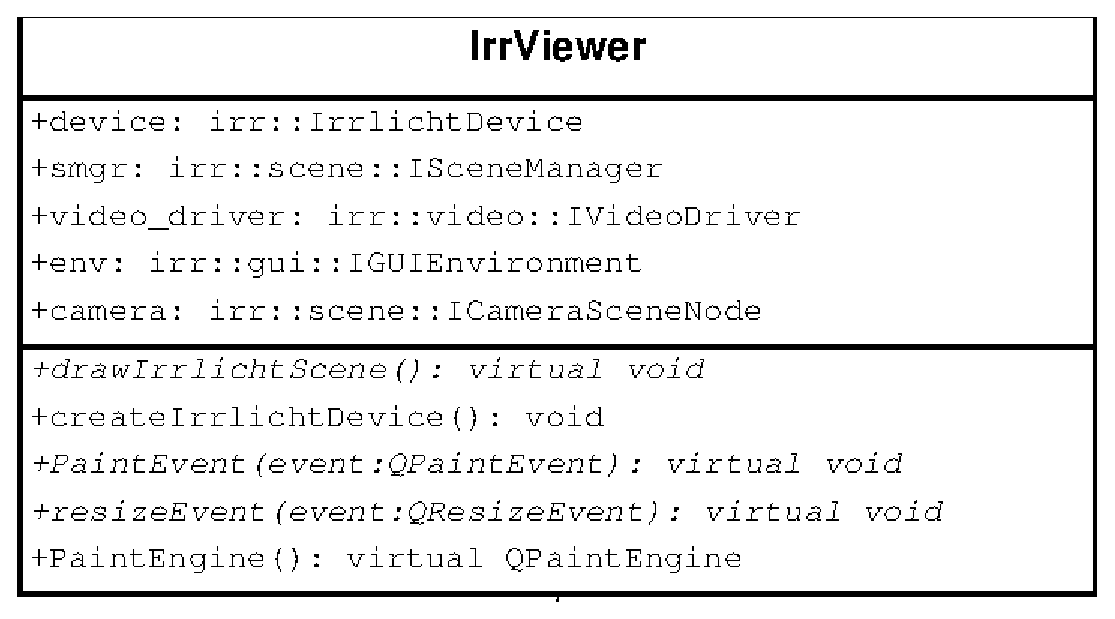
\includegraphics[scale = 0.4]{classeirrviewer}
	\caption{Classe IrrViewer.}
	\label{fg:classeirrviewer}
\end{figure}

	Assim, com o \textit{Qt-Creator} reconhecendo essa nova classe como uma de suas janelas(Widget), pode-se passar para segunda fase do projeto (desenvolvimento de outras classes e métodos necessários para preenchimento dos requisitos pré-estabelecidos).

	A classe MyReceiverEvent(Fig.~\ref{fg:classereceiverevent}) foi criada com intuito de comunicar o  evento de \textit{mouse} do \textit{Qt} com a \textit{engine Irrlicht}. Desta forma, quando este evento for disparado ( chamado ), passará para o objeto desta classe o estado do \textit{mouse} que será tratado e enviado para o \textit{Irrlicht}. 
\begin{figure}[!ht]
	\centering
	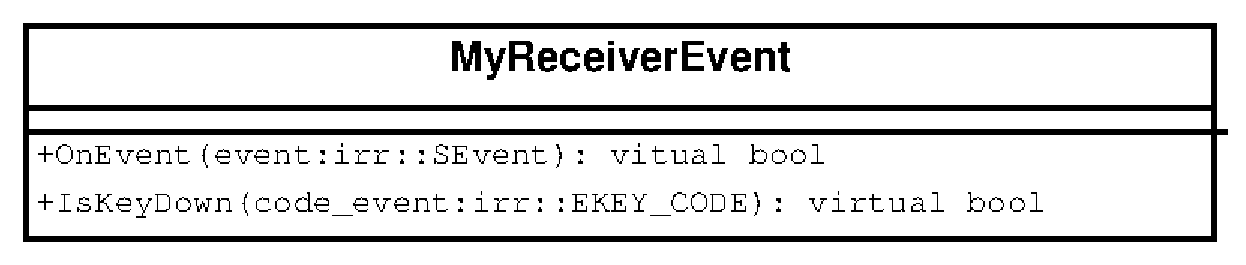
\includegraphics[scale = 0.4]{classereceiverevent}
	\caption{Classe ReceiverEvent.}
	\label{fg:classereceiverevent}
\end{figure}

	O papel de dar suporte à criação de objetos tridimensionais para o cenário virtual foi designado a classe \textit{IrrNode} (Fig.~\ref{fg:classeirrnode}). Portanto esta contém a implementação dos métodos de construção dos todos os objetos 3D básicos suportados pela interface criada neste trabalho, tais como os de criação de cubos, esferas, hastes, cilindros e cones.
\begin{figure}[!ht]
	\centering
	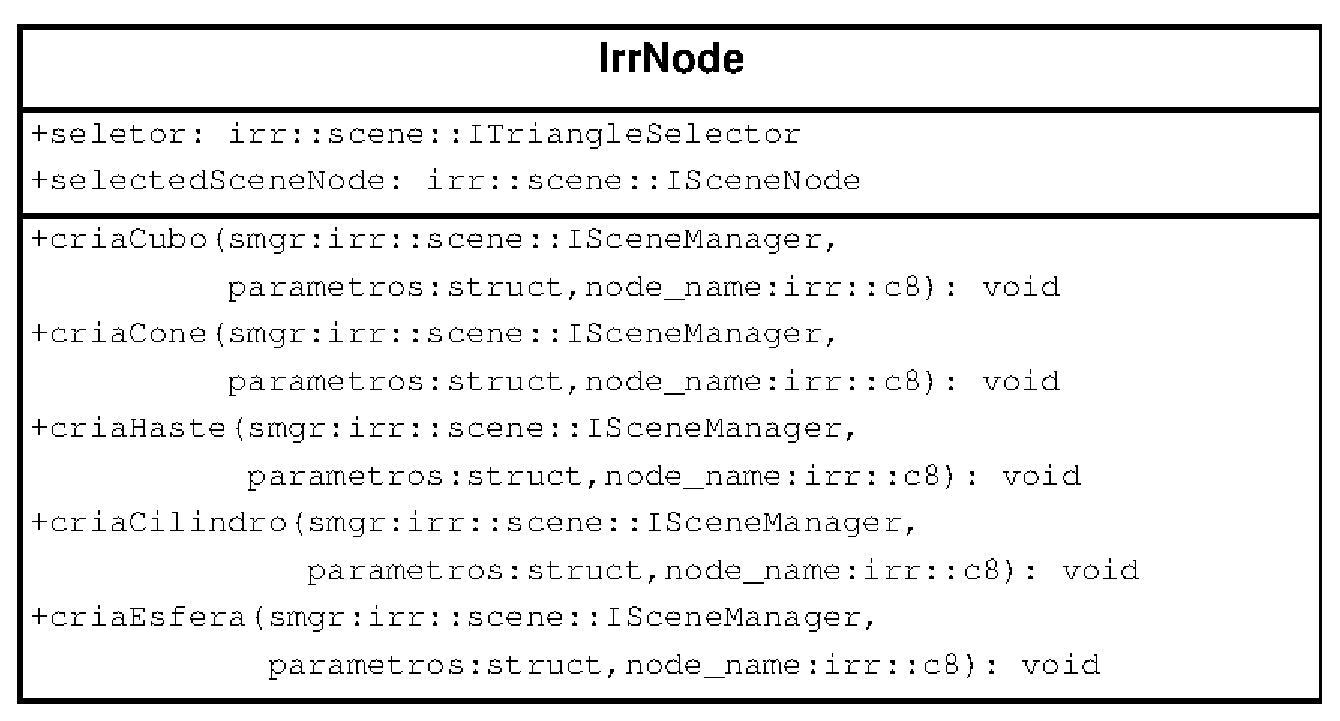
\includegraphics[scale = 0.4]{classeirrnode}
	\caption{Classe IrrNode.}
	\label{fg:classeirrnode}
\end{figure}

	Já os atributos e métodos necessários para modificação do cenário virtual estão presentes na classe \textit{Cena}~(\ref{fg:classecena}). Sendo ela, desta forma, a responsável pelo gerenciamento de todo e qualquer evento que ocorra dentro do AV. Ela faz isso, utilizando-se dos : objetos das classes \textit{IrrNode} e \textit{MyReceiverEvent}, dos métodos herdados da classe \textit{IrrViewer} (olhar Figura~\ref{fg:classes}) e dos seus próprios métodos e atributos. 
\begin{figure}[!ht]
	\centering
	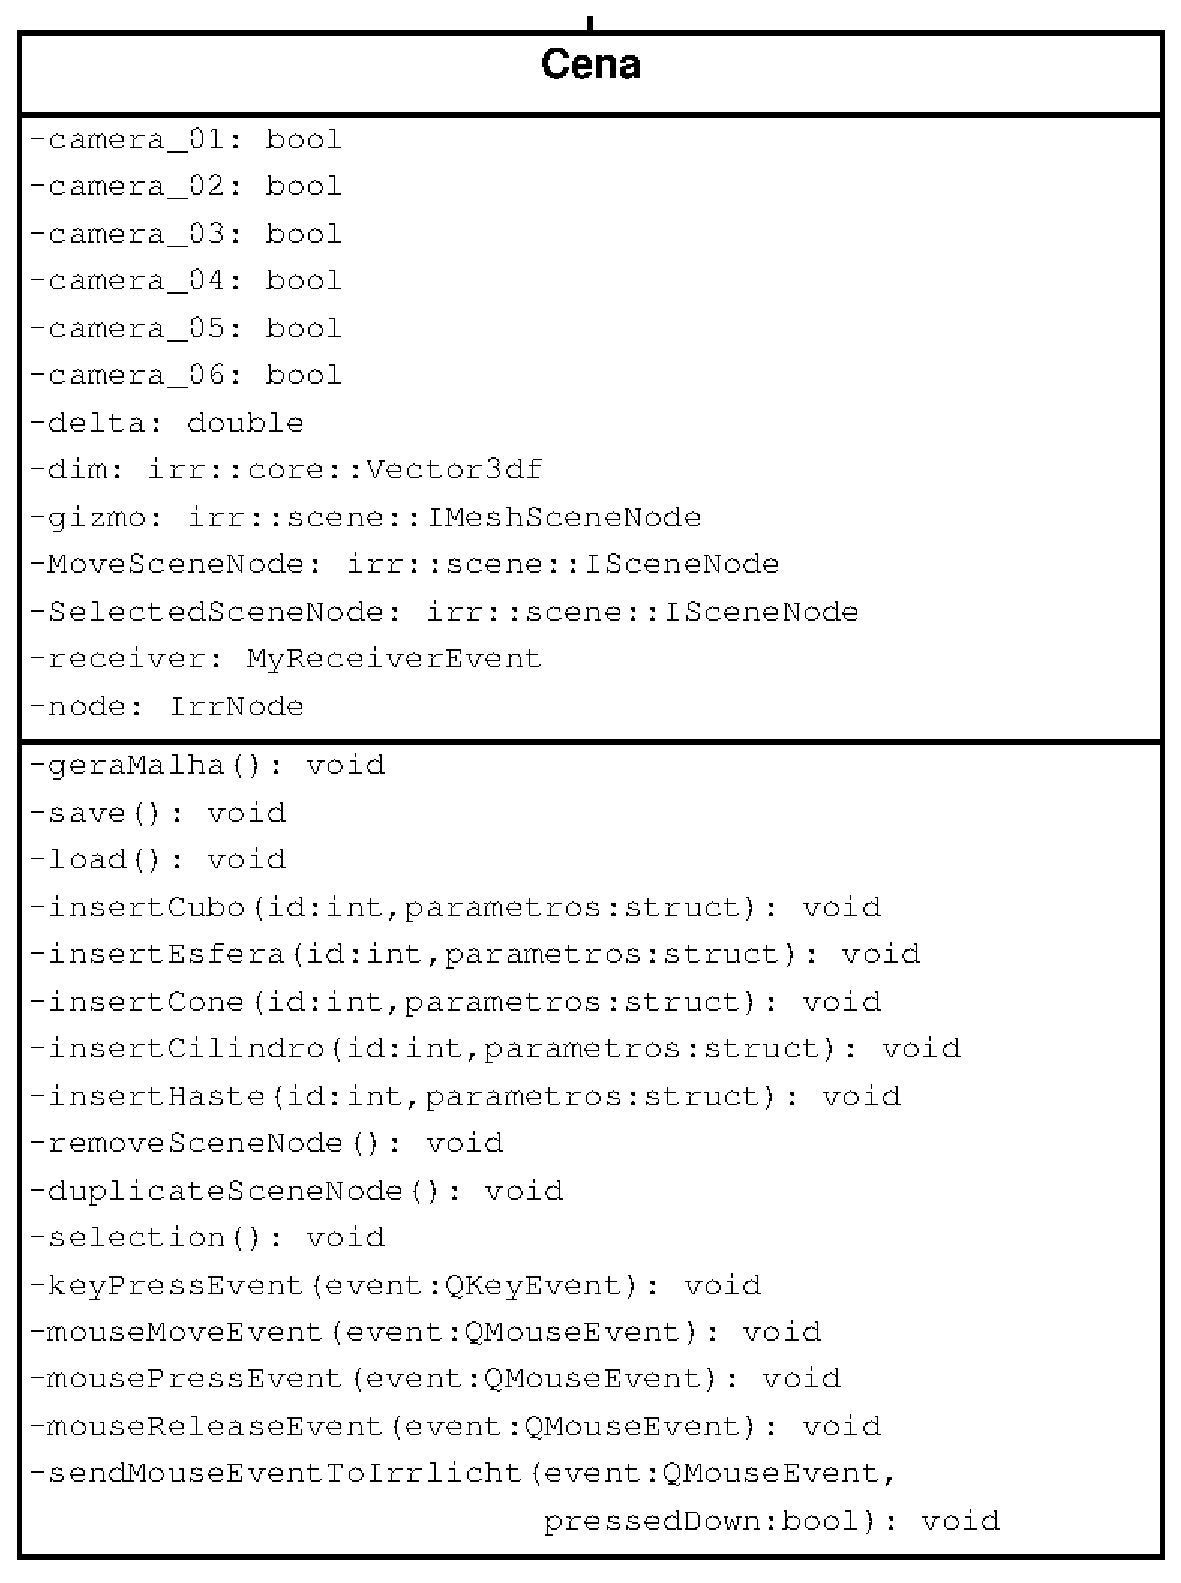
\includegraphics[scale = 0.4]{classecena}
	\caption{Classe Cena.}
	\label{fg:classecena}
\end{figure}

	Por fim, temos a classe \textit{MainWindow}, que utiliza-se de um objeto da classe \textit{Cena} para comunicar as alterações realizadas na interface com a janela {Irrlicht} e vice-versa. Desta forma, fazendo o tratamentos dos eventos de botão, mudança nos valores  dos  painéis laterais e dos campos de posição e rotação. A Figura~\ref{fg:classemainwindow} mostra os principais atributos e métodos deste classe.
\begin{figure}[!ht]
	\centering
	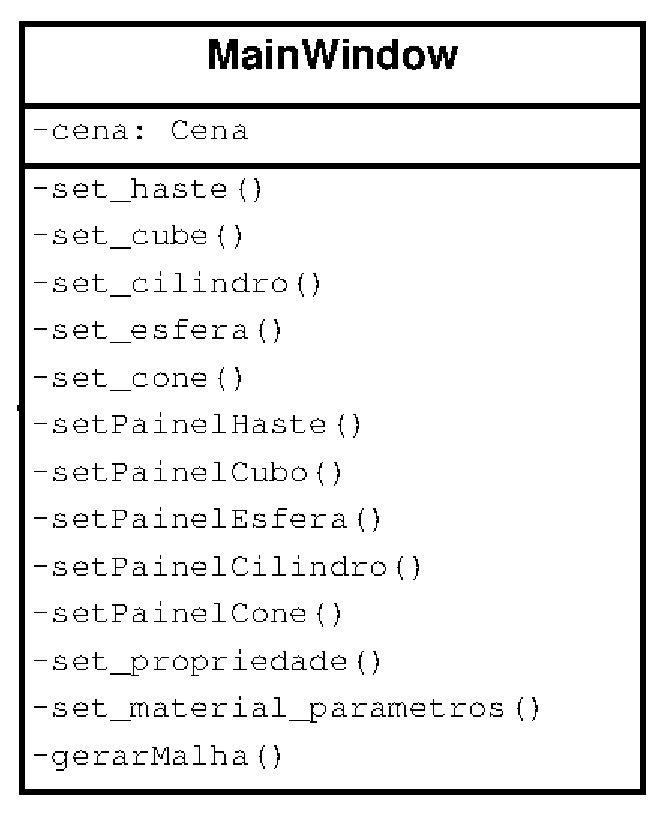
\includegraphics[scale = 0.4]{classemainwindow}
	\caption{Classe \textit{Mainwindow}.}
	\label{fg:classemainwindow}
\end{figure}

\section{Interface}
	O software desenvolvido neste projeto está ilustrado na Figura~\ref{fg:layout}. Seu layout e suas ferramentas foram baseada nos softwares de modelagem mais utilizados no mercado, que são: Blender, 3DStudio e Maya. A sua estrutura foi dividida em 4 áreas: barra superior, janela da cena, painéis laterais e barra inferior.
\begin{figure}[!ht]
	\centering
	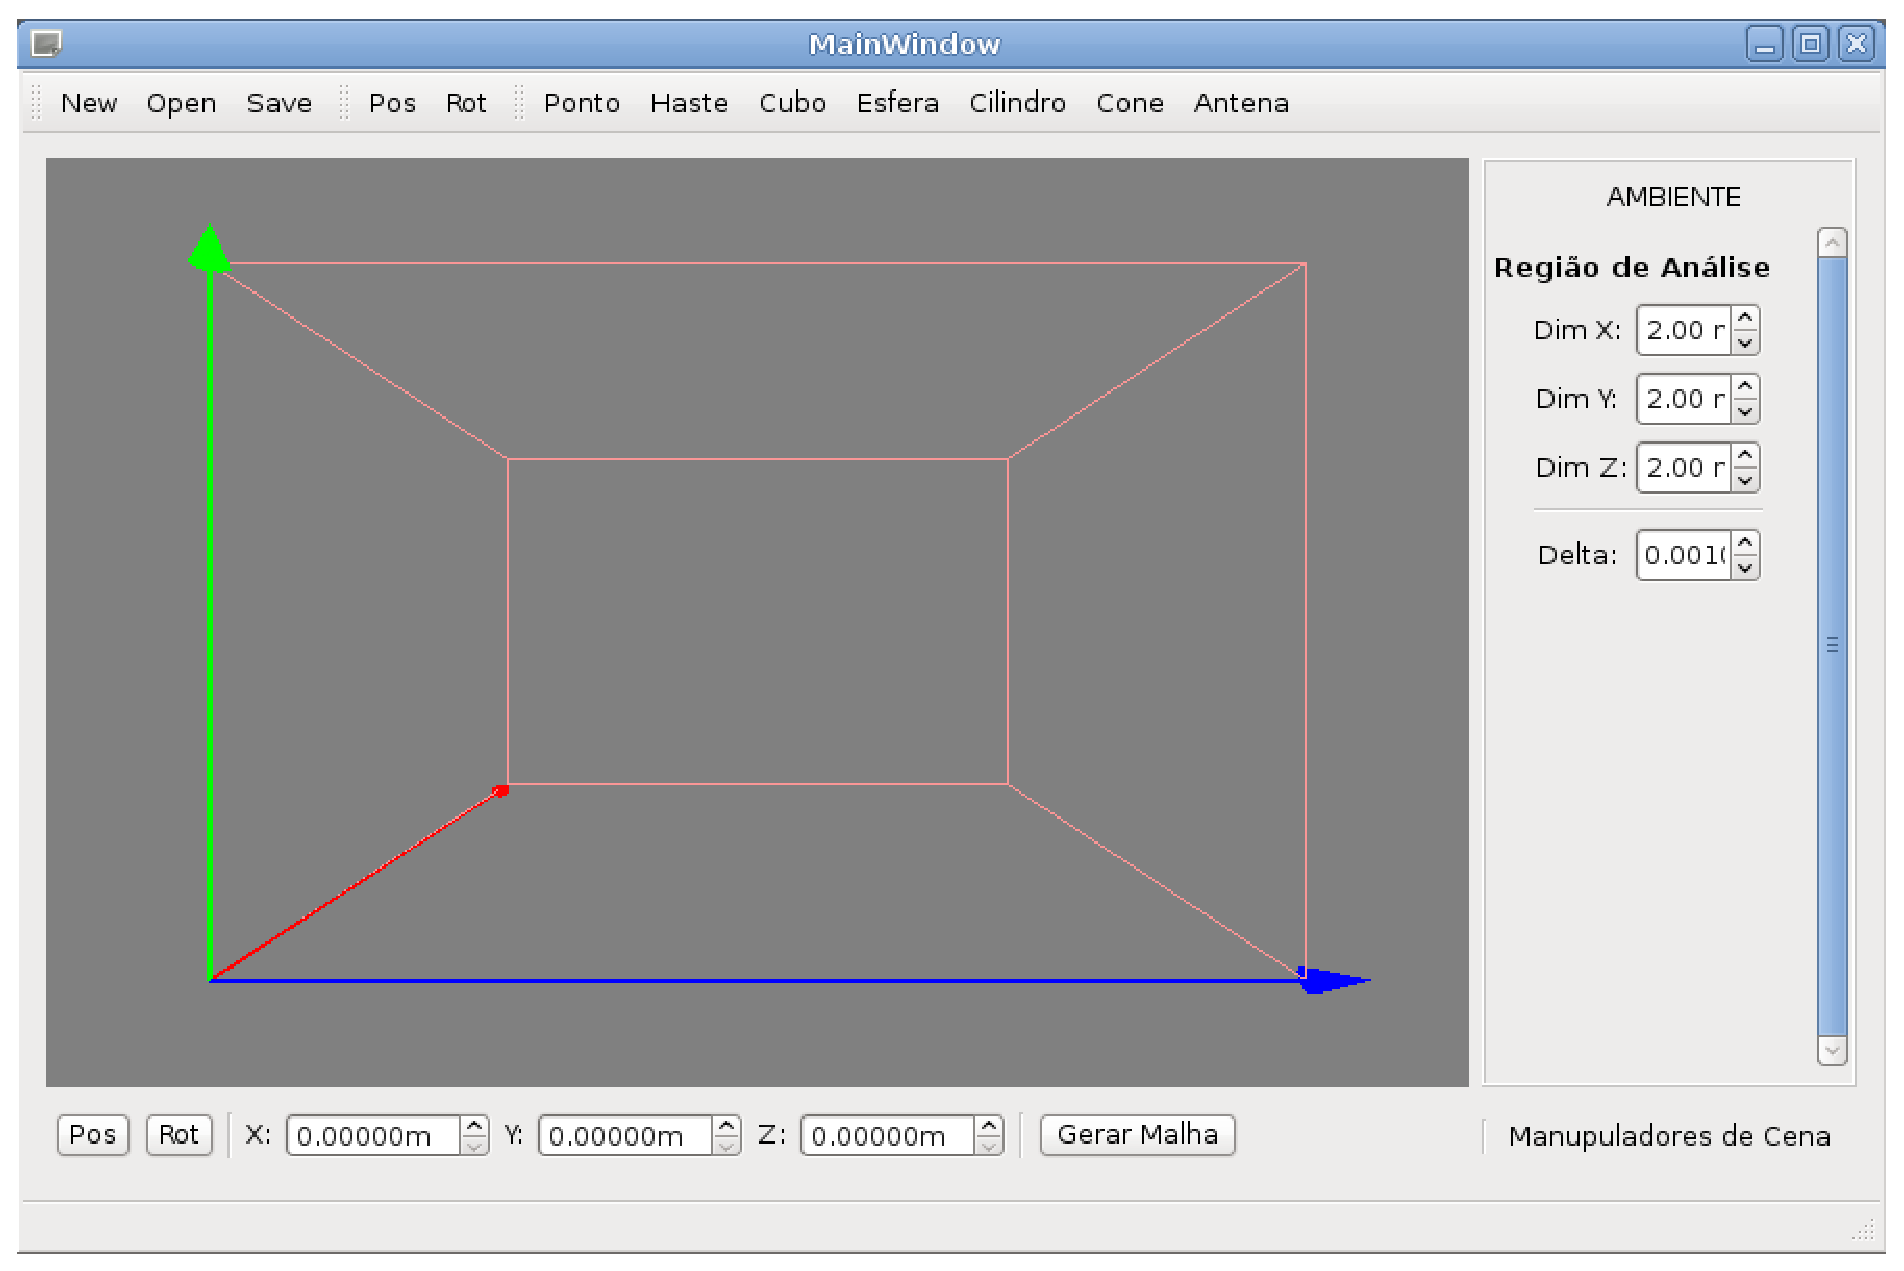
\includegraphics[scale = 0.4]{layout}
	\caption{Layout da interface.}
	\label{fg:layout}
\end{figure}

	Na barra superior, Figura~\ref{fg:barra_s}, encontra-se primeiramente o botão \textit{New}, que tem o propósito de criar uma nova cena \textit{Irrlicht}. Quando pressionado, ativa uma janela (Figura~\ref{fg:dados_r}) que requisita os dados necessários para criação da região de análise, tais como valores de dimensionamento (tamanho em $x$, $y$ e $z$) e o valor do $delta$ (dimensão da célula de Yee). Em seguida vem o botão \textit{Open}, que carrega uma cena anteriormente salvada (caso exista). Depois dele tem-se o botão \textit{Save}, que salva a cena atual em uma arquivo chamado \textit{Map.in}, que contém todas as características dos objetos (tamanho, tipo e parâmetros físicos), assim como suas posições.

\begin{figure}[!ht]
	\centering
	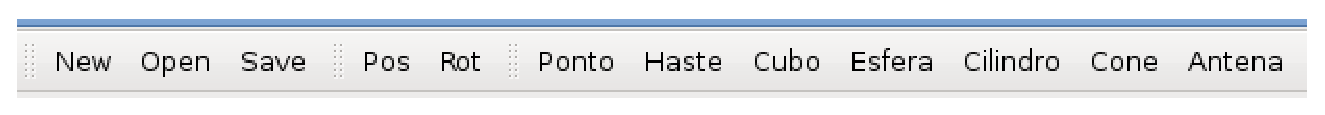
\includegraphics[scale = 0.4]{barra_s}
	\caption{Barra Superior interface.}
	\label{fg:barra_s}
\end{figure}
\begin{figure}[!ht]
	\centering
	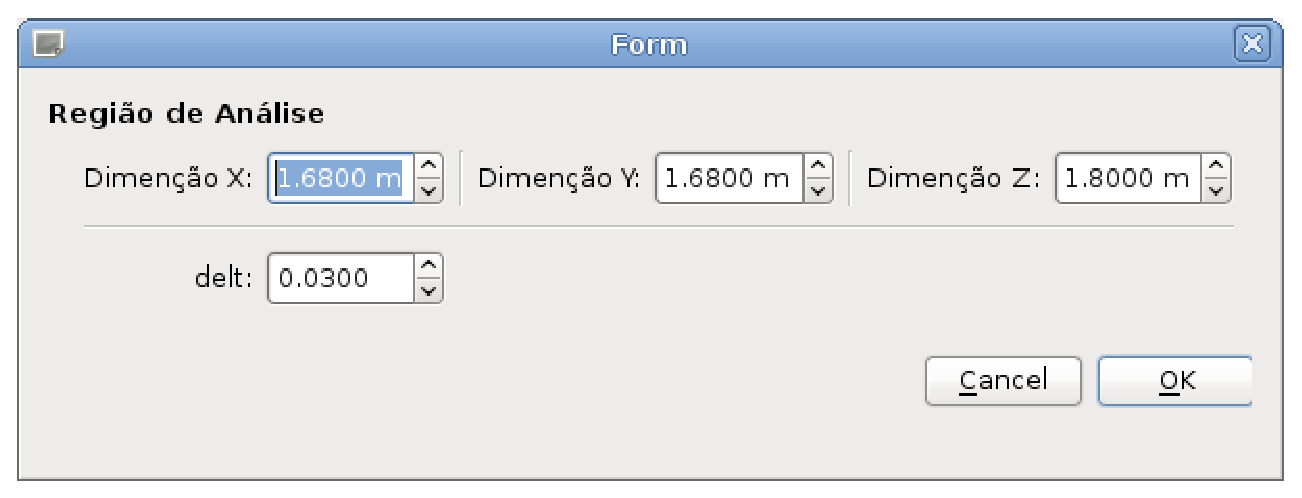
\includegraphics[scale = 0.4]{dados_r}
	\caption{Janela com as característica da região de análise.}
	\label{fg:dados_r}
\end{figure}

	Mas em frente, encontram-se os botões \textit{Pos} e \textit{Rot}, os quais dão suporte à visualização e manipulação do posicionamento e dos ângulos de cada objeto selecionado, respectivamente. Logo em seguida encontram-se os criadores de objetos básico da interface, que são \textit{Ponto},\textit{Haste}, \textit{Cubo}, \textit{Esfera}, \textit{Cilindro}, \textit{Cone} e por fim \textit{Antena}. Quando ativados criam o objeto desejado com a posição e os parâmetros previamente especificados.

	A janela da cena, Figura~\ref{fg:janela_c} é uma região do software onde se visualiza o universo virtual. Nesta região, é possível realizar manipulações através do mouse como seleção, translação e rotação. Ela está diretamente relacionada a classe \textit{IrrViewer}, pois é uma instância (objeto) desta classe. 

\begin{figure}[!ht]
	\centering
	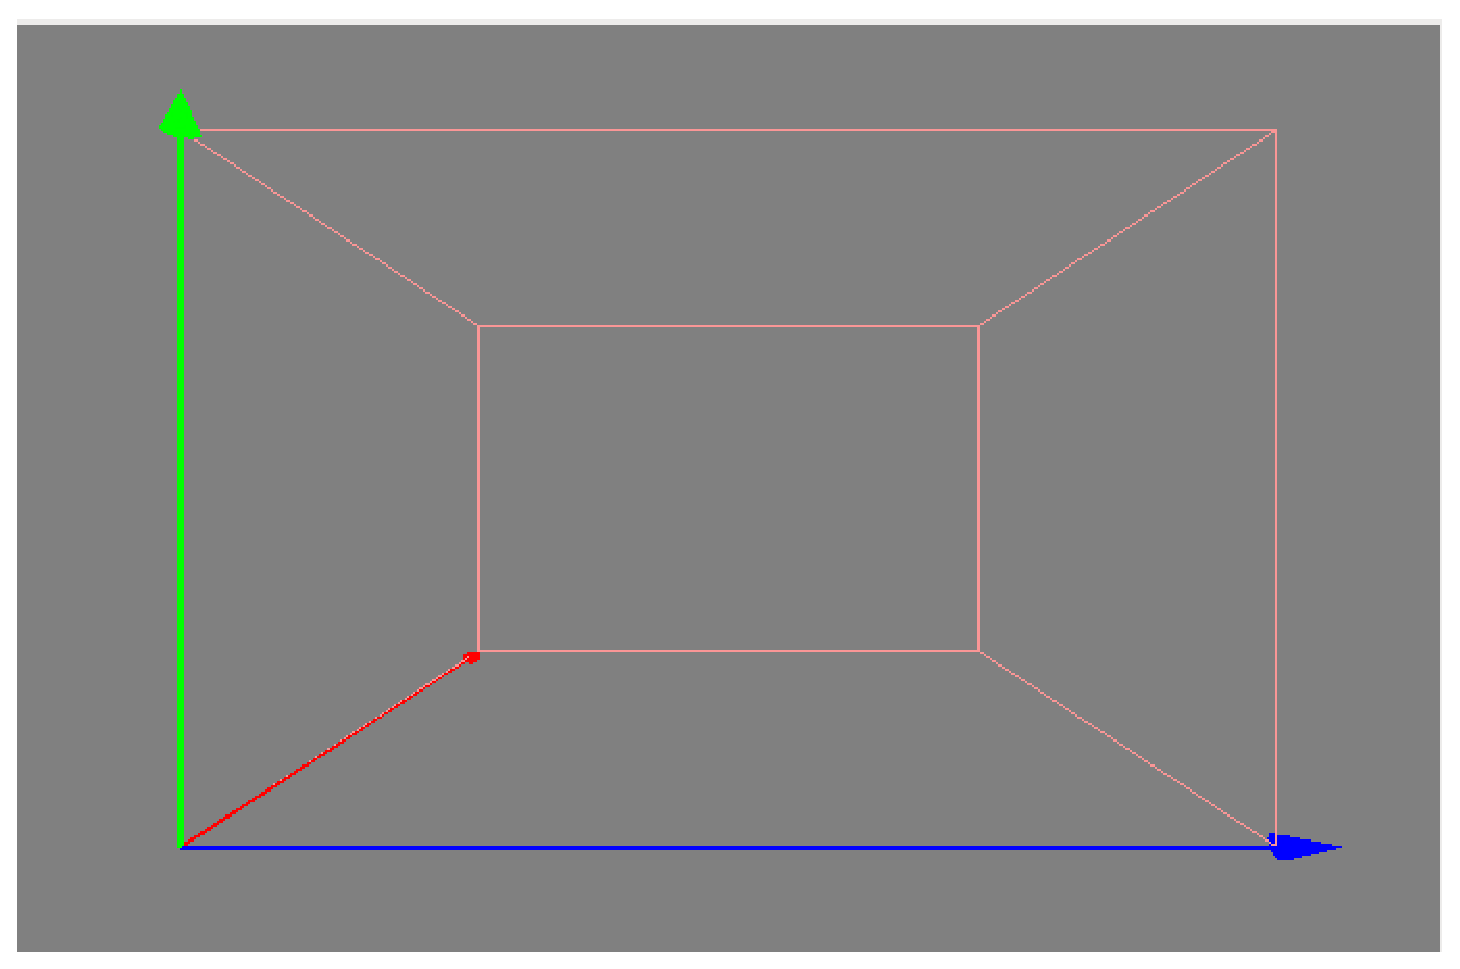
\includegraphics[scale = 0.4]{janela_c}
	\caption{Janela da Cena.}
	\label{fg:janela_c}
\end{figure}

	O painel lateral, Figura~\ref{fg:painel_l} é uma área de visualização e manipulação das características relacionadas ao tamanho e parâmetros físicos dos objetos.

\begin{figure}[!ht]
	\centering
	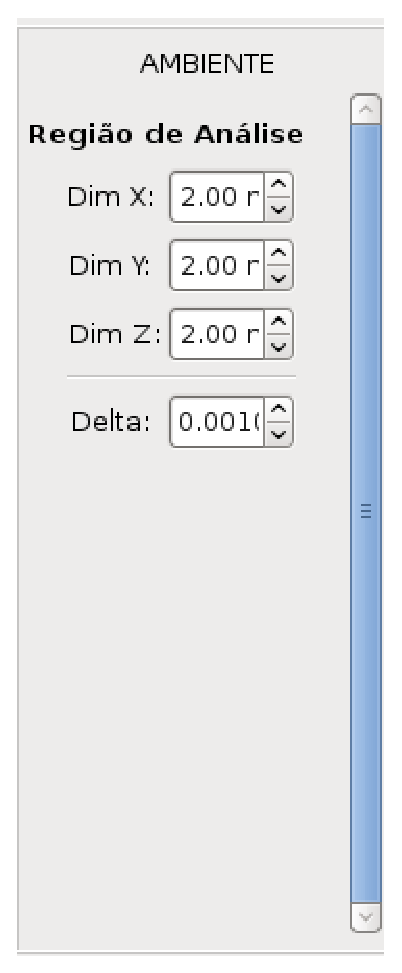
\includegraphics[scale = 0.4]{painel_l}
	\caption{Painel lateral dos parâmetros da região de análise.}
	\label{fg:painel_l}
\end{figure}

	Na parte inferior da interface(Figura~\ref{fg:barra_i}) encontram-se os botões \textit{Pos} e \textit{Rot}, que têm as mesmas funcionalidades dos já citados da barra superior. Em seguida  há um conjunto de itens que possibilitam a visualização e manipulação das coordenadas relativas a posição e rotação do objeto selecionado ($X$, $Y$ e $Z$). E por fim, o botão \textit{gerar Malha}, o qual tem a função de gerar e salvar a malha representativa de todos os  objetos construídos no cenário virtual.

\begin{figure}[!ht]
	\centering
	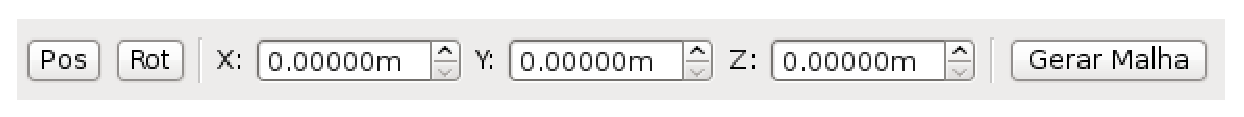
\includegraphics[scale = 0.4]{barra_i}
	\caption{Barra inferior da interface.}
	\label{fg:barra_i}
\end{figure}

\section{Funcionalidades}
	\subsection{Atalhos de Teclado}
	A facilidade de navegação e manipulação, são características fundamentais para qualquer software de modelagem. Os atalhos de teclado são criados com o intuito de reduzir esforço e tempo do usuário. Esta ferramenta é um conjunto de teclas que ao serem pressionadas realizam uma ação. As ações realizadas pelas teclas de atalho, normalmente podem ser realizada por outras ferramentas como botões, menus, etc.
	
	A Tabela~\ref{tb:shortcuts} contém todos os atalhos de teclado criados para este projeto.

\begin{table}
\centering
\begin{tabular}{|l|l|}
	\hline
		Atalho & Funcionalidade \\ \hline
		Shift+O &  Afastamento\\ \hline
		Shift+P &  Aproximação\\ \hline
		W & Focaliza objeto selecionado\\ \hline
		C & Clona objeto selecionado(duplica)\\ \hline
		R & Remove objeto selecionado \\ \hline
		1 & Muda para câmera frente \\ \hline
		2 & Muda para câmera lateral esquerda \\ \hline
		3 & Muda para câmera lateral direita \\ \hline
		4 & Muda para câmera traseira \\ \hline
		5 & Muda para câmera topo \\ \hline
		6 & Muda para câmera base \\ \hline
		M + X & Permite movimentação de objeto selecionado no eixo X com o mouse \\ \hline
		M + Y & Permite movimentação de objeto selecionado no eixo Y com o mouse \\ \hline
		M + Z & Permite movimentação de objeto selecionado no eixo Z com o mouse \\ \hline
		Shift + A & Permite movimentação de objeto selecionado nos eixos X e Y com o mouse \\ \hline
		Shift + B & Permite movimentação de objeto selecionado nos eixos X e Z com o mouse \\ \hline
		Shift + C & Permite movimentação de objeto selecionado nos eixos Y e Z com o mouse \\ \hline
		Shift + D & Permite movimentação de objeto selecionado nos eixos X, Y e Z com o mouse \\ 
	\hline
\end{tabular}
\caption{Tabela de Atalhos de teclado.}
\label{tb:shortcuts}
\end{table}
	
\subsection{Eventos de Colisão}
\label{sec:colisao}
	Os eventos de colisão possibilitam que duas ou mais formas geométrica existentes no AV possam colidir.  Neste trabalho utilizou-se a colisão por reta, que é ortogonal ao plano de visualização da câmera. Seu ponto inicial fica posicionado no centro ecrã (tela), já seu o ponto final é deslocado do inicial por uma distância consideravelmente maior do que qual uma das arestas da região de análise. Este ponto final responde ao evento de \textit{mouse}, ou seja, no caso da ocorrência de um \textit{click}  em um determinado ponto do cenário 3D a reta de colisão terá o seu ponto inicial recebendo o valor central da tela e o final obtendo o valor da posição do \textit{mouse}.  No caso de esta reta encontrar (colidir) algum objeto entre seus pontos ele será o objeto selecionado. 
 
	Para diferenciar, visualmente, objetos selecionados dos não selecionados, utilizou-se da técnica de representação \textit{wireframe}. Portanto, quando ocorrer um evento de colisão e um objeto é selecionado, a visualização deste objeto muda, passando a ser representado somente por suas arestas e vértices. A Figura~\ref{fg:colision} demostra este fato.
\begin{figure}[!ht]
	\centering
	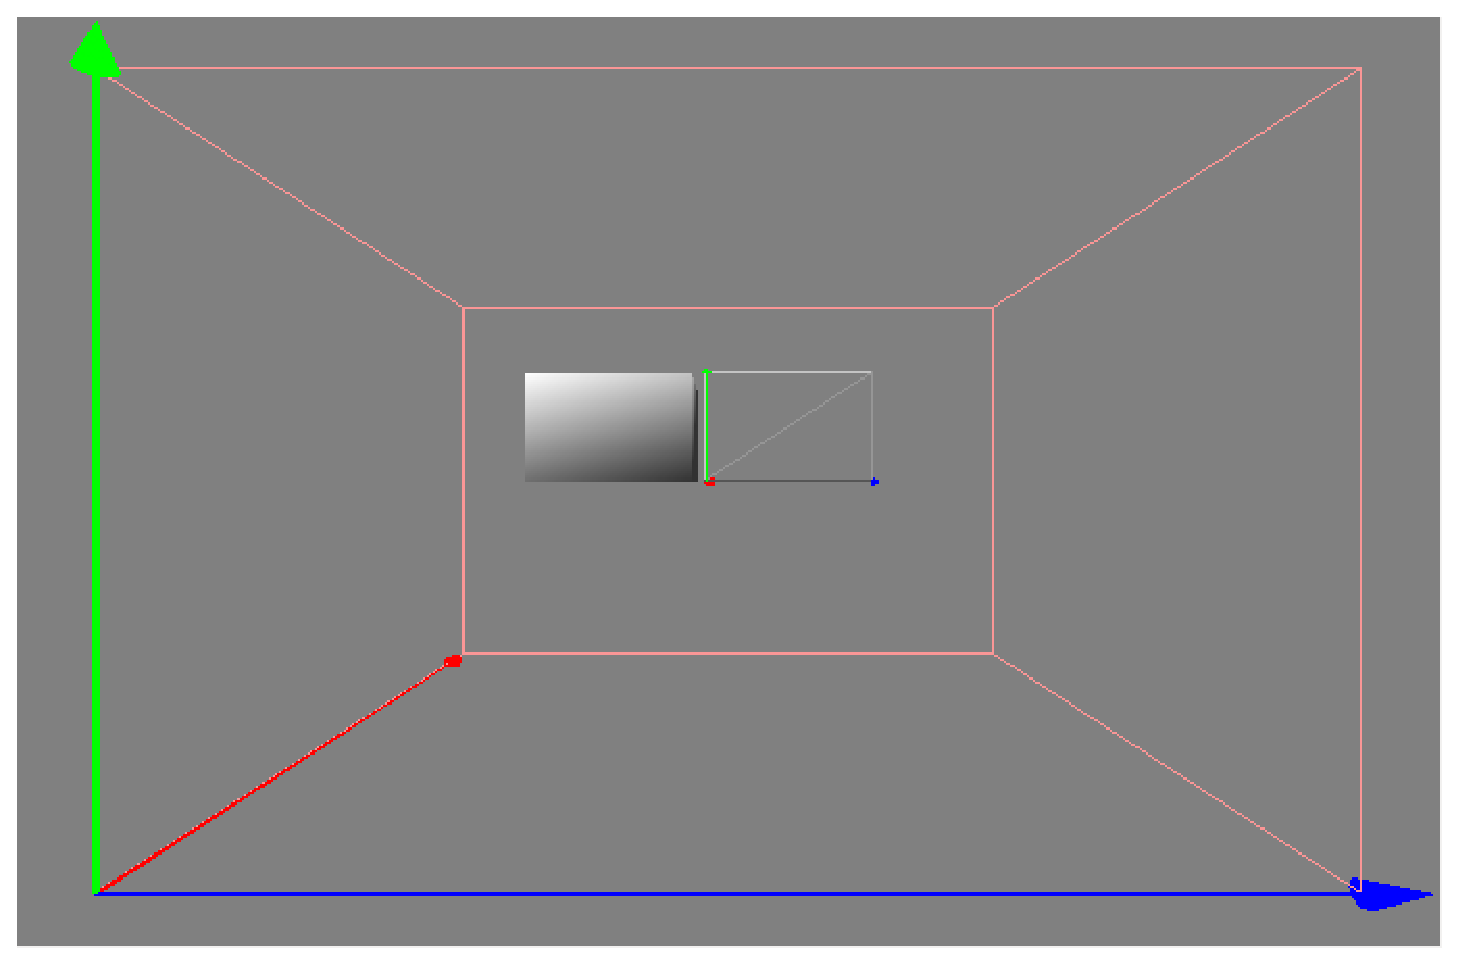
\includegraphics[scale = 0.4]{colision}
	\caption{Ilustração do evento de colisão com o objeto cubo.}
	\label{fg:colision}
\end{figure}

\subsection{Visualizações}
	A possibilidade de visualização de um cenário por vários ângulos é fundamental quando se está modelando um ambiente 3D, principalmente quando o cenário modelado será utilizado em simulações eletromagnéticas, onde qualquer erro estrutural poderá gerar resultados não desejados (sem sentido). Para sanar esse problema, o software confeccionado neste projeto, permiti visualizar o AV por seis câmeras diferentes: frontal(padrão), lateral esquerda, lateral direita, traseira, topo e base. 

\subsection{Aproximação e Afastamento}
	Tem a finalidade de, juntamente com as seis visualizações possíveis(seis câmeras diferentes), facilitar a navegação e alteração do cenário virtual. Sendo uma ferramenta importante na modelagem, por permitir a aproximação e afastamento de um determinado região ou objeto selecionado dentro do ambiente virtual. As teclas de atalho associadas a aproximação são $Shift+P$ ou $W$ e as associadas aos afastamento são $Shift+O$.

	As figuras a seguir ilustram o uso desta ferramenta. A Figura~\ref{fg:nor} mostra um objeto a uma distância padrão (sem afastamento ou aproximação). Na Figura~\ref{fg:afas} pode ser visto o mesmo objeto após um determinado afastamento (utilizando $Shift+O$). Já as Figuras~\ref{fg:apr} e \ref{fg:w} mostra os efeitos da  aproximação normal (usando o atalho $Shift+P$) e a por seleção (dada pela tecla $W$).

\begin{figure}[!ht]
	\begin{center}
		\subfigure[Visualização de objeto cilindro sem aproximação, afastamento ou mudança de foco da câmera.]{\label{fg:nor}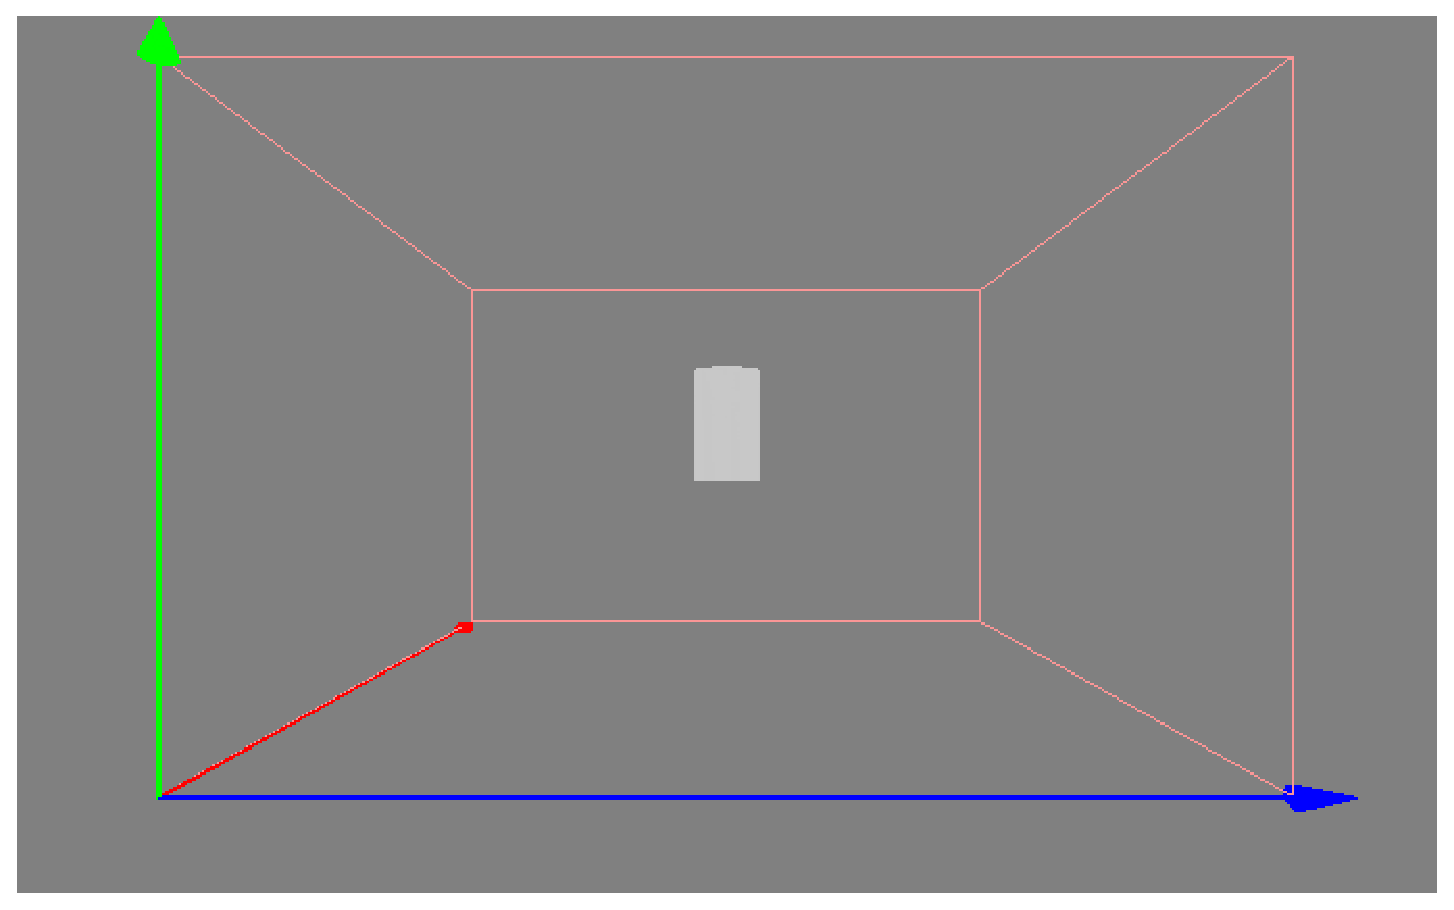
\includegraphics[scale=0.25]{nor}}
\qquad
		\subfigure[Visualização de objeto cilindro com afastamento.]{\label{fg:afas}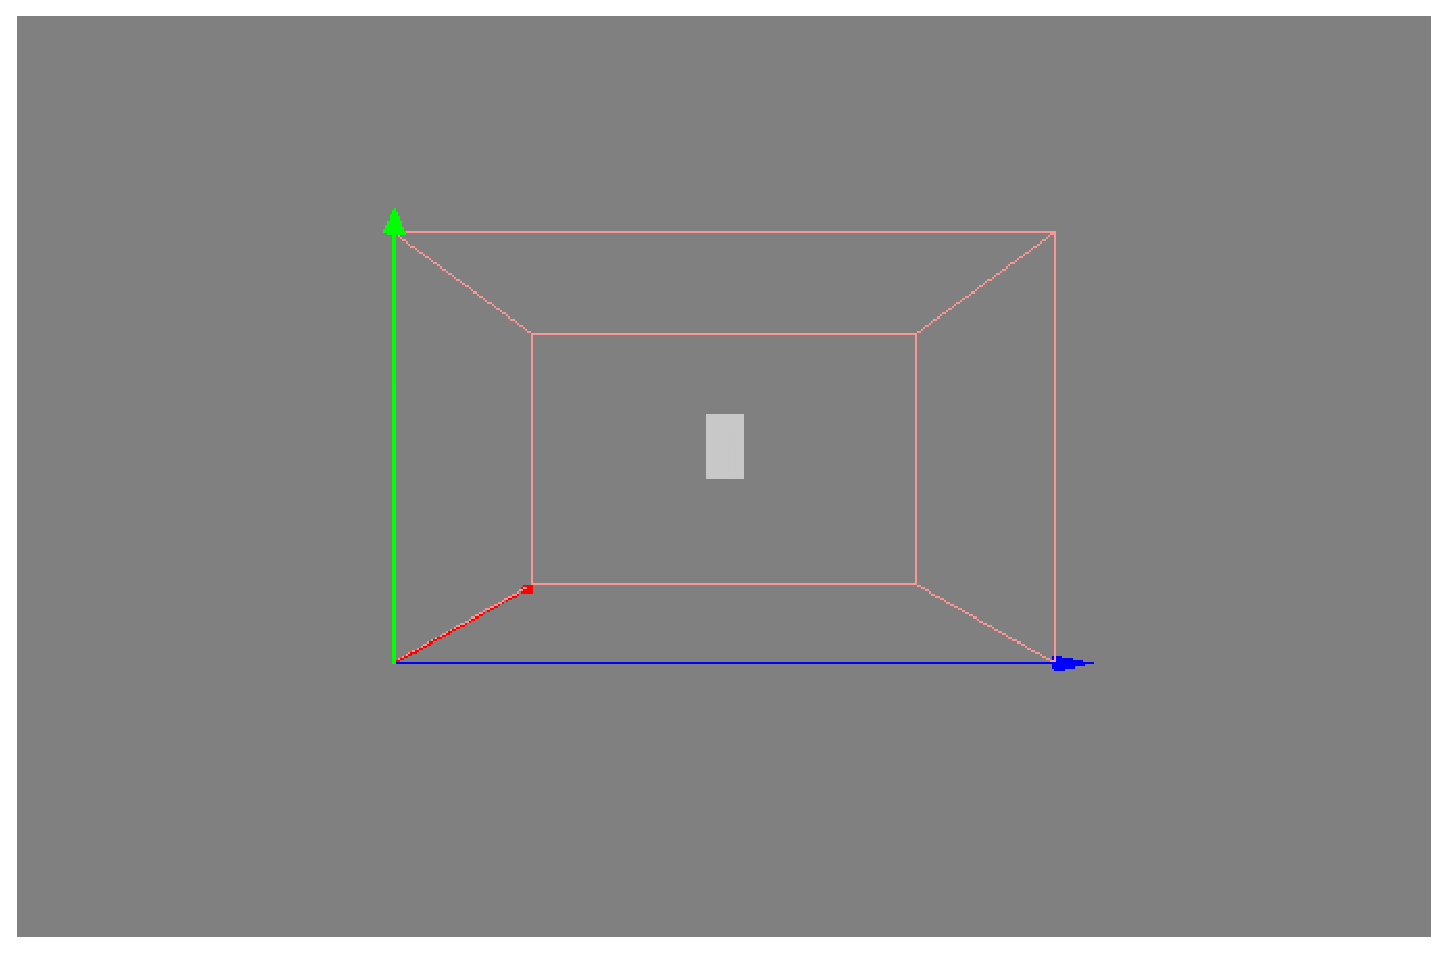
\includegraphics[scale=0.25]{afas}}
	\end{center}
	\caption{Visualização por afastamento.}
	\label{fg:afastamento}
\end{figure}

\begin{figure}[!ht]
	\begin{center}
		\subfigure[[Visualização de objeto por aproximação normal(sem mudança de foco).]{\label{fg:apr}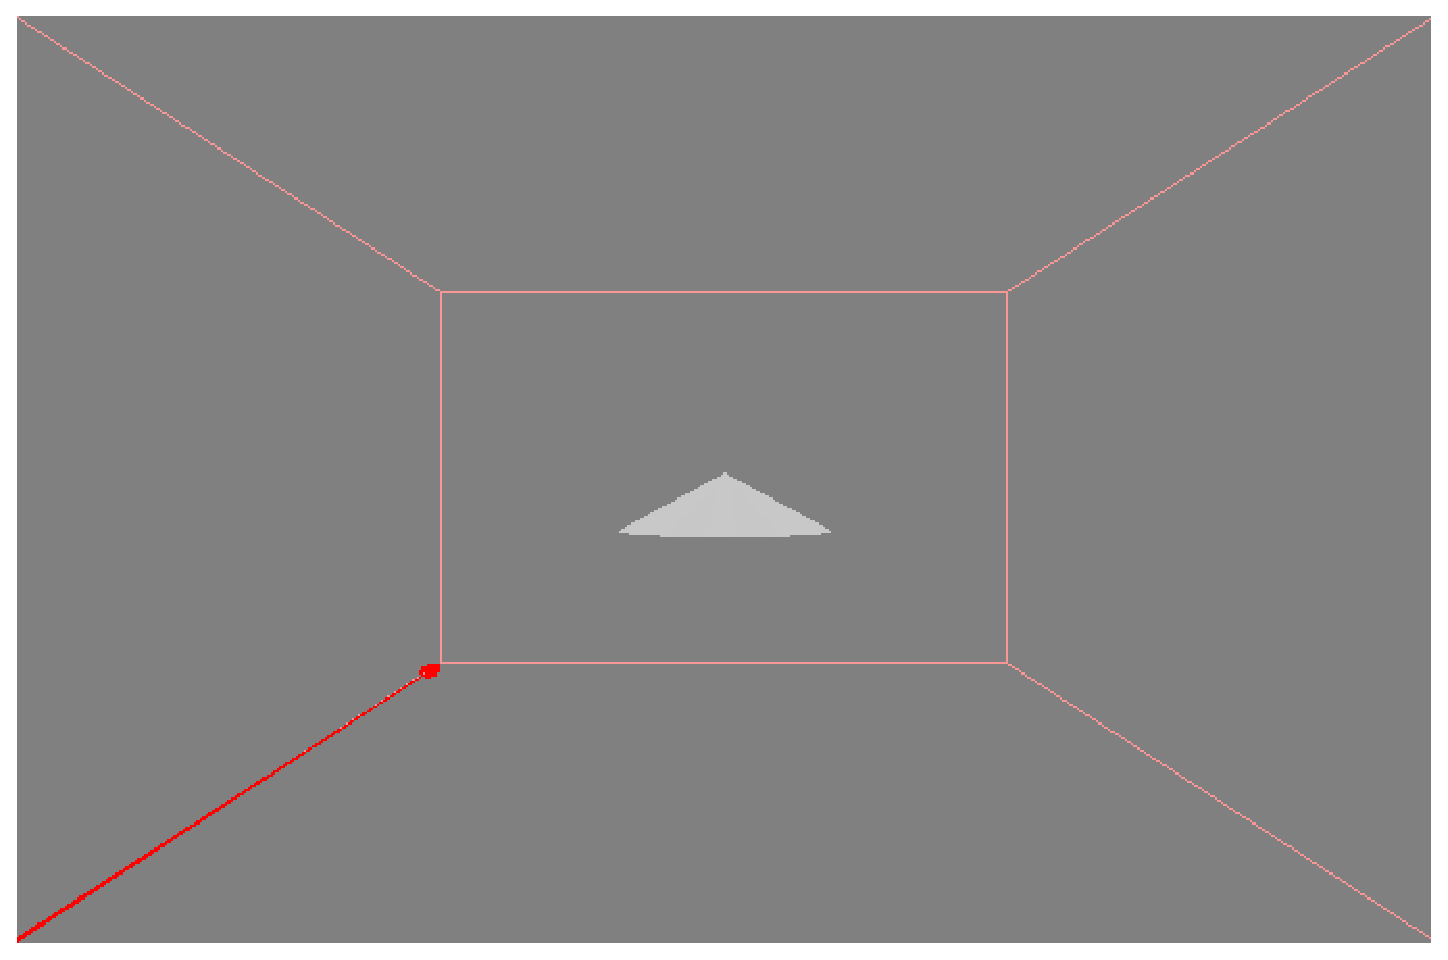
\includegraphics[scale=0.25]{apr}}
\qquad
		\subfigure[Focalização de objeto selecionado através da tecla $W$.]{\label{fg:w}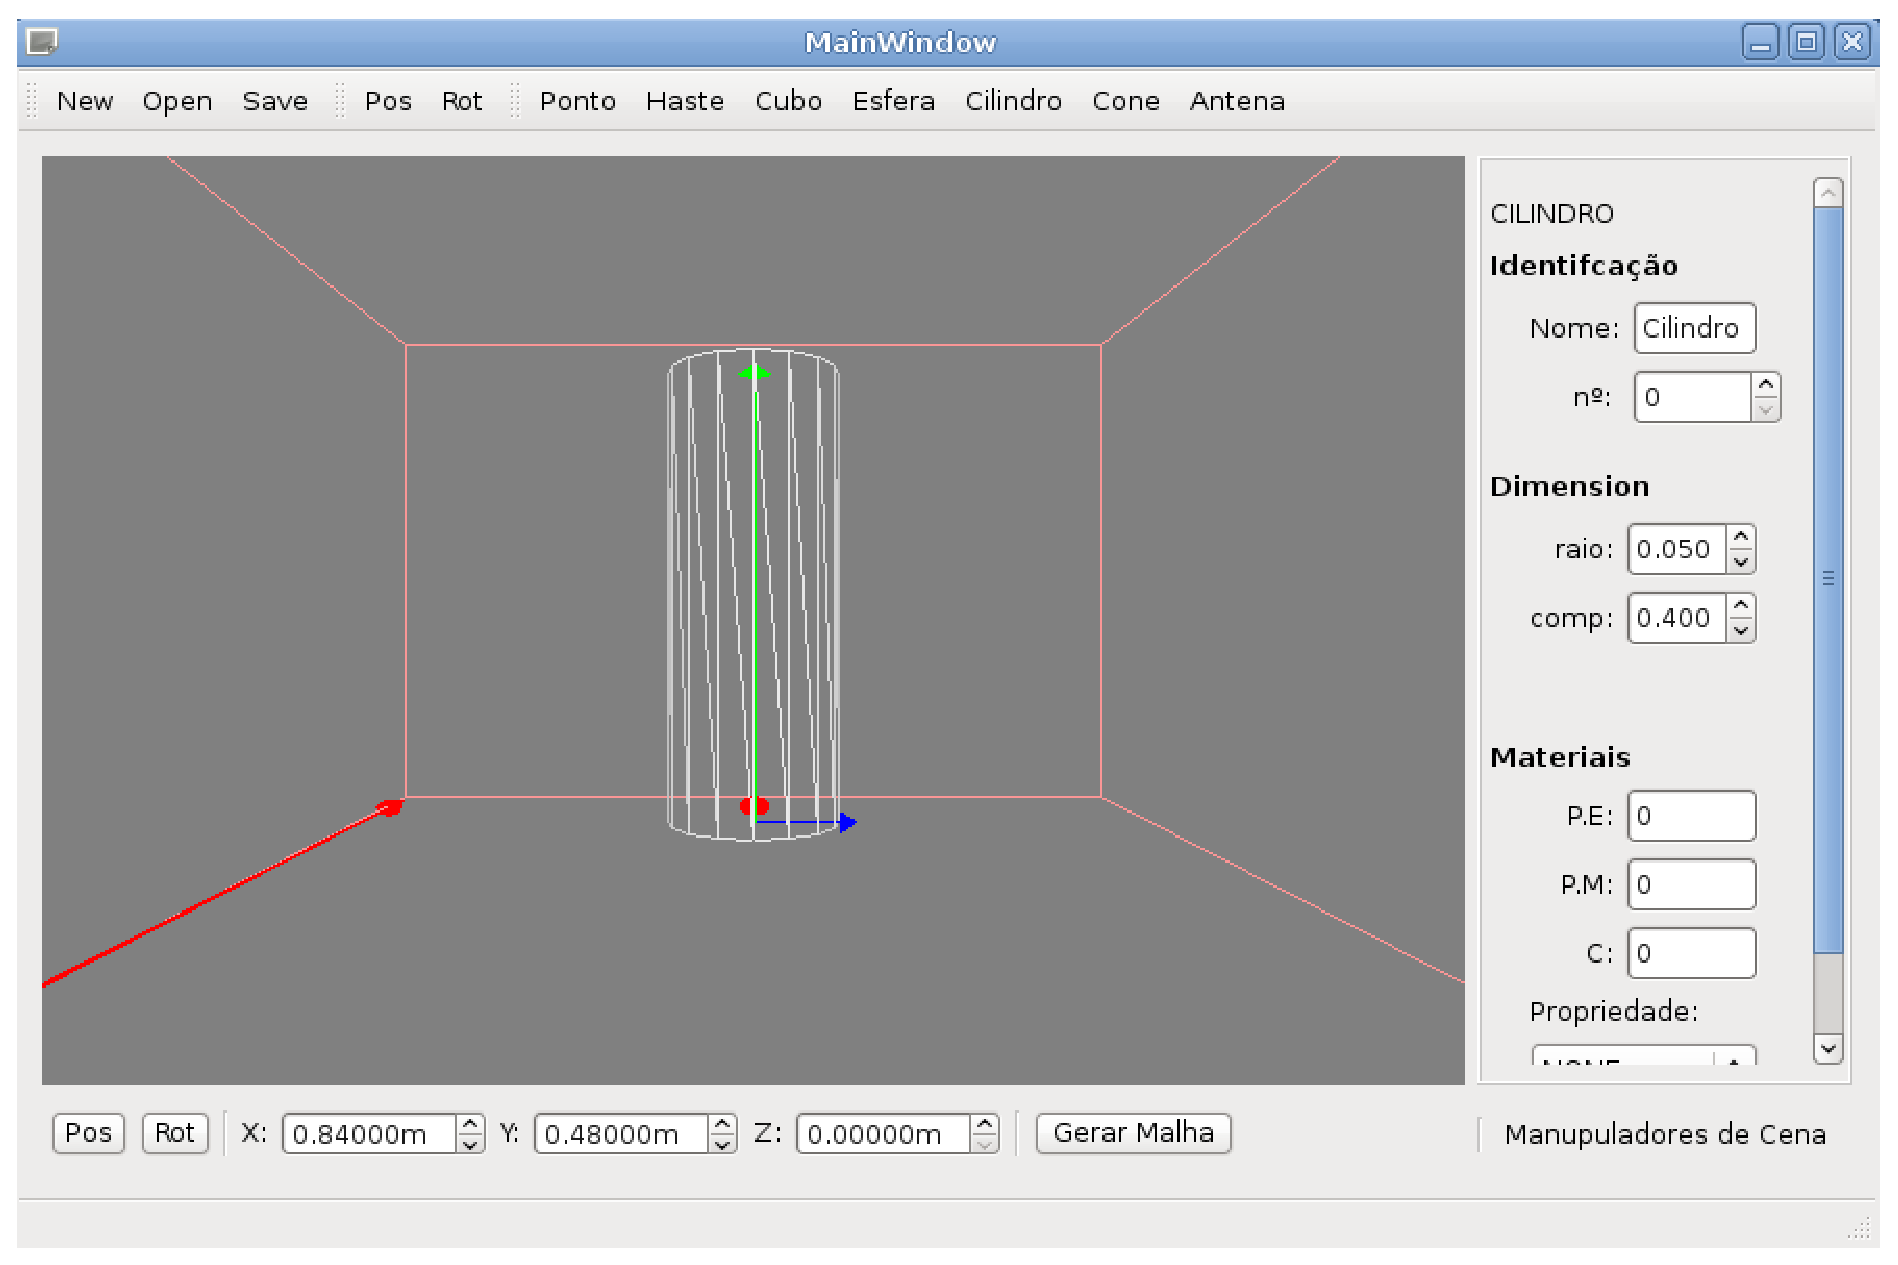
\includegraphics[scale=0.25]{w}}
	\end{center}
	\caption{Visualização por aproximação.}
	\label{fg:aproximacao}
\end{figure}

\subsection{Conexão com o LANE-SAGS}
\label{sec:c_sags}
	Depois de implementar todas as funcionalidades do software, passou-se para o último requisito proposto para este projeto, a conexão com o simulado LANE-SAGS. Esta conexão foi realizada por meio de dois arquivos.

	O primeiro arquivo é o bd.in (bd - bloco dielétrico), que contém os prismas retangulares (células) que representam, por enumeração de ocupação espacial, os objetos contínuos modelados na interface. A sequência de gravação de cada prismas no arquivo segue a forma: célula inicial $X$, célula final $X$, célula inicial $Y$, célula final $Y$, célula inicial $Z$, célula final $Z$, $\epsilon_r$, $\sigma$ e $\mu_r$.
 Além do arquivo bd.in, é gerado um segundo arquivo chamado \textit{simconf.in}(simconf- configuração da simulação) contendo as informações referentes às: dimensões das células de Yee (em metros) e a dimensão em células do Espaço Delimitador (região de análise).
Com os arquivos gerados e a conexão estabelecida, basta inserir (utilizando o LANE-SAGS) alguns fatores fundamentais para efetuar uma simulação de propagação eletromagnética, tais como: antena, planos de visualização, fonte e corrente. O diagrama mostrado na Figura \ref{fg:c_sags}, ilustra o processo de execução de uma simulação utilizando os dois softwares.

\begin{figure}[!ht]
	\centering
	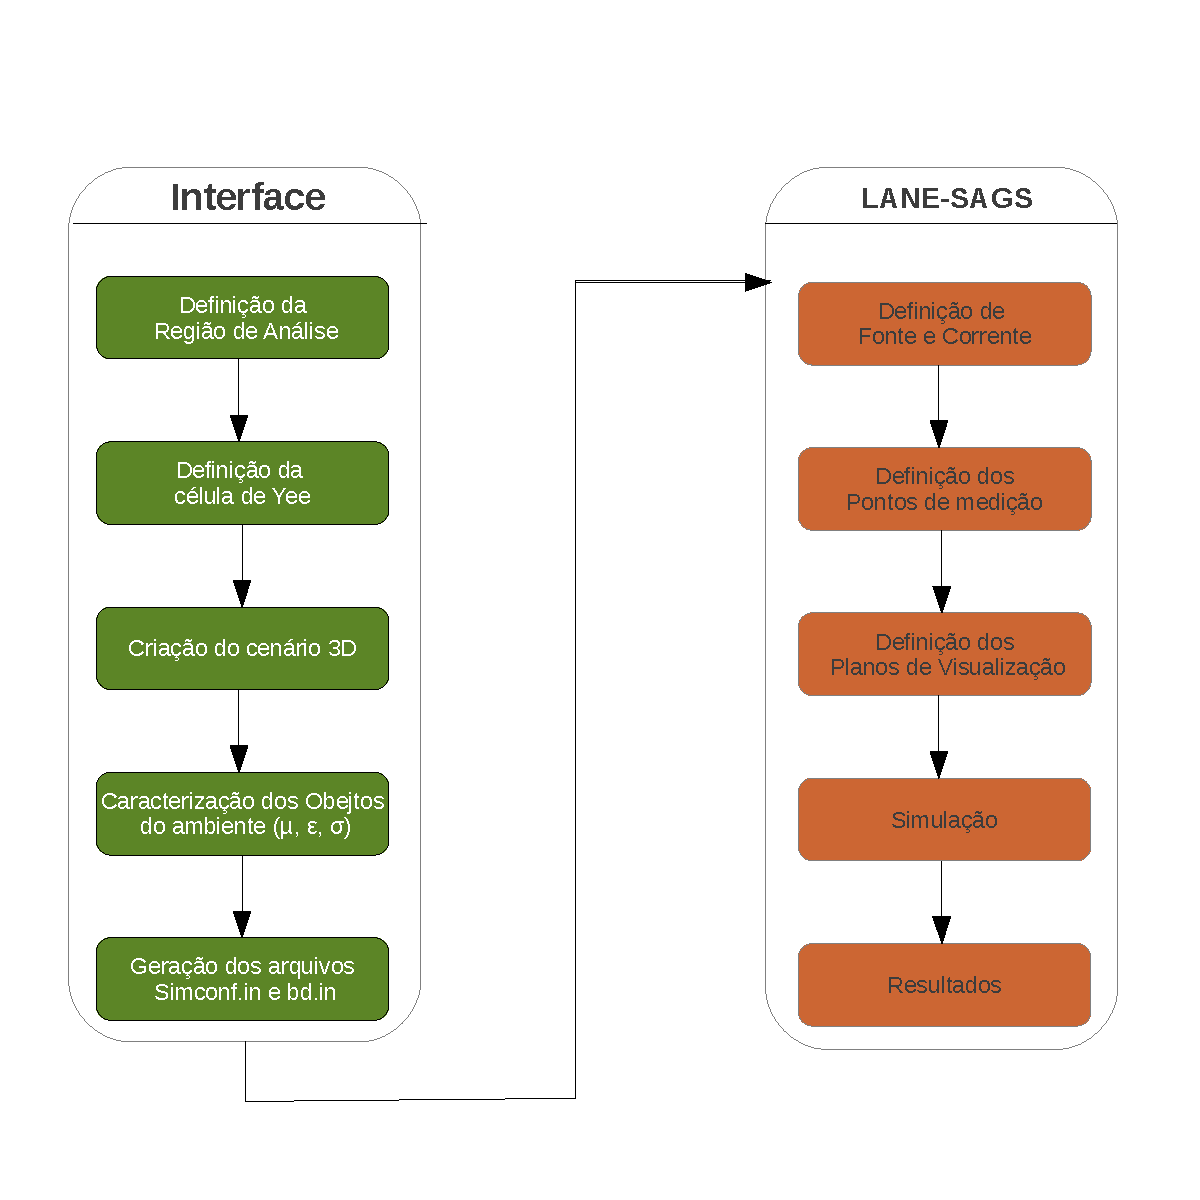
\includegraphics[scale = 0.8]{c_sags}
	\caption{Diagrama de conexão com o LANE-SAGS.}
	\label{fg:c_sags}
\end{figure}
